\documentclass[printmode]{mgr}

\usepackage[utf8]{inputenc}
\usepackage[T1]{fontenc}

\usepackage{pdflscape}

% https://www.sharelatex.com/learn/Paragraph_formatting
\setlength{\parindent}{0mm}
\setlength{\parskip}{2ex}

% https://en.wikibooks.org/wiki/LaTeX/Source_Code_Listings
\usepackage{listings}
\lstset{
  frame=single,
  numbers=left,
  breaklines=true,
  postbreak=\mbox{$\hookrightarrow$\space}
}

\usepackage{graphicx}
\usepackage{caption}
\usepackage{subcaption}
\usepackage{psfrag}
\graphicspath{{./images/}}

\usepackage{amsmath}
\usepackage{amsfonts}

\usepackage{supertabular}
\usepackage{array}
\usepackage{tabularx}
\usepackage{hhline}

\usepackage{hyperref}

\title{Embedded Linux \\ build systems}
\engtitle{Systemy implementacji \\ wbudowanego Linuxa}
\author{Cezary Dynak}
\supervisor{dr Witold Paluszyński}

\field{Automatyka i~Robotyka (AIR)}
\specialisation{Embedded Robotics (AER)}

\begin{document}
%\bibliographystyle{plabbrv}
\bibliographystyle{plabbrv}

\maketitle
\dedication{6cm}{To my wife and son}

\tableofcontents




















\chapter{Introduction}
% important note - idea of this chapter - not goals, but "tasks to be done" / "the main problems to be solved" - explain title, describe it more precisely 

The main task of this work is to describe and compare tools, that help in the process of creating and deploying Linux-based operating system on embedded devices.
There are many publications, that prioritize one build system or are focused on low-level problems common for all, but there was a lack of treating them as one type of software.
I'm trying to fill this gap and encourage everybody who is working with embedded Linux, to give a try for all presented tools.

It's also worth to emphasize, that this topic is not limited to hobby projects and academic research, but it's essential for commercial and industrial applications.
Since nowadays micro-controllers are much more powerful and enormously cheaper than yesterday's supercomputers, the main focus has moved from resources optimization to convenient maintaining.
Growing costs of employment are also forcing companies to shorten time to market with the use of existing software components, especially free and open source ones.
The overwhelming use of Linux in modern embedded devices, instead of traditional bare-metal programming, is shown on the Figure \ref{fig:iot-os}.

\begin{figure}[htbp]
  \centering
    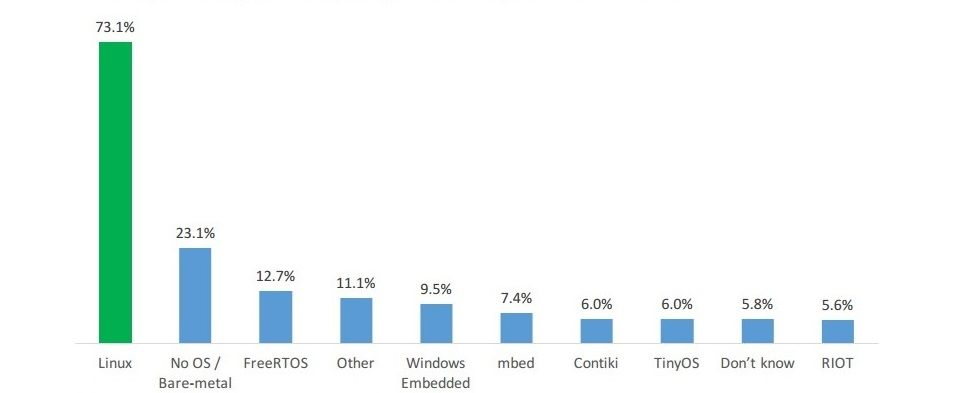
\includegraphics[width=\textwidth]{iot-os.jpg}
    \caption{Survey results for Operating Systems used for IoT Devices\cite{web:iot-os}}
  \label{fig:iot-os}
\end{figure}


\section{Basic definitions}
% TODO: add bibliography sources

Despite that every aspect of computing could be described by numbers and mathematical operations, there could be plenty of definitions for one and the same thing. Unfortunately the naming conventions are sometimes misleading, as it is in the area which I am describing. People understand the word ``Linux'' differently in different contexts, as there is also the never ending debate about the term ``GNU/Linux''.\cite{web:gnu-linux} Sometimes buzzwords like ``cloud'' and ``IoT'' are strongly promoted due to commercial issues, which makes common understanding even more unclear. Therefore, I would like to explain how to interpret the key wording.

\paragraph{Operating system} is a software that manages hardware resources and provides interface to run other programs.\cite{web:def-os}

\paragraph{Operating system kernel} is a core part of operating system, that provides  basic low level interfaces.\cite{web:def-kernel}
% Implementing Operating Systems without Kernels ???
% https://dl.acm.org/citation.cfm?id=902543

\paragraph{Linux} is an open source operating system kernel, that was inspired by the Unix tradition. The initial release took place in 1991 and since then it is being developed by thousands of voluntary collaborators as well as major IT companies. Formerly it was compatible only with the x86 standard processors for personal computers, but now it is available for other architectures, especially ARM that is used by most mobile and embedded devices. The work of its creator Linux Torvalds and lead maintainer Greg Kroah-Hartman is currently sponsored by the Linux Foundation. As for 2018, all of the world fastest supercomputers from TOP 500 ranking are using this kernel.

\paragraph{Linux distribution} is the operating system, that is built upon the Linux kernel.
% is using the Linux kernel? - be careful with i.e. "Windows subsystem for Linux" case

% \paragraph{Note:} Based on those definitions we could say that $kernel \le OS$, so $Linux < OS$ or $Linux = OS$ depending on case.

\paragraph{Embedded device} is a micro-controller based device, that has a fixed purpose and strictly limited user interface.

\paragraph{Cross-compiler} is a compiler that creates executable code for system architecture that is different from its own.

\paragraph{Embedded Linux build system} is a set of software development tools, that create Linux distribution with the use of cross-compiler and produce complete operating system image, to be deployed on an embedded device.

The umbrella them ``Embedded Linux build system'' is not widely in use, but despite the similarities between described tools, no other was proposed. Different projects identify themselves as ``distribution creators'' or ``executable documentation'', but they share the same goal and they need to be compared in one place.

\section{Sources of knowledge}
\label{section:sources-of-knowledge}

There are two important issues, that I faced while trying to make literature review: firstly what kind of materials should I analyze and secondly how to extend my searches, to get a full overview of current state of knowledge on this topic.

The first issue was very clear in the previous (20th) century - making literature review was mostly limited to analyzing two kind of printed materials: longer ones which were just scientific books and shorter ones which were peer reviewed articles in technical journals.
Right now they are also available and easy accessible in electronic form and still they are the most reliable sources for literature review, but not every IT engineer is using it.
Open Source Software and Open Source Hardware movement, beside creating lot of tools, also created a lot of written knowledge, but they are distributed in very different ways: project documentation, presentations, tutorials, source code comments, READMEs, How Tos, FAQs, wikis, finally blog and forum posts, but also in other forms.
Because they are all available via Internet, there exists one unified way to reference them: URL (Unified Resource Locator) also known as web address or link.
Because of that, this and most of other bibliographies are filled with URLs, not ISBNs.

The second thing is how to be sure that I covered every aspect, at least by mentioning. Search results are personalized, both by behavior of searcher, that is choosing keywords and also Search Engine Optimization.
Nobody could tell, that this is complete, but sources are cross referenced, so after some research, the loop closes.
Most important factor for choosing materials is their universality and chance that they will be not so fast outdated.

\subsection*{elinux.org}

The Embedded Linux Developer wiki elinux.org is undeniably the most extensive source of knowledge about all aspects of Embedded Linux.
In this form it was possible to consolidate a powerful community which extend its contents.
From one side it is greatly filled with a lot of technical details and still extended, but from the other the materials are not always universal and some pages are not maintained.

The elinux.org domain was registered on 1999-11-04 \cite{web:whois-elinux} and used by the Linux specialist Tim Riker just as a placeholder.\cite{web:riker}\cite{web:elinux-placeholder}
About 2003 the Embedded Linux wiki was initiated here using the MoinMoin framework \cite{web:elinux-moinmoin}.
In 2007 it was moved to the Media Wiki engine, that is still in use.
On the top level, its contents are divided into two main parts: ``Development Portals'' about various aspects of embedded Linux and ``Hardware Pages'' for different development boards.
The most relevant page for this thesis is \url{http://elinux.org/Build_Systems}, but build systems are only listed there without any comparison.

Currently it is maintained by the Core Embedded Linux Project which belongs to Linux foundation \cite{web:linuxfoundation-celp}.
CELP is also the coordinator of other important Embedded Linux activities.

\subsection*{wikipedia.org}
% http://dbpedia.org/page/Category:Embedded_Linux
% http://dbpedia.org/page/Linux_on_embedded_systems

Wikipedia allows anyone to edit articles, so professionalism of every page can not be assured, but it is the largest and most popular general reference work on the Internet.
The most important thing from my point of view, is that it redirects and groups abstract entities on a high level.
The Table \ref{table:wikipedia} summarizes pages that are most relevant for this work.

\begin{table}
  \begin{tabular}{| l | l |}
    \hline
    \url{https://en.wikipedia.org/wiki/Category:Embedded_Linux} & \\
    \hline
    \url{https://en.wikipedia.org/wiki/Category:Software_related_to_embedded_Linux} & \\
    \hline
    \url{https://en.wikipedia.org/wiki/Category:Embedded_Linux_distributions} & \\
    \hline
    \url{https://en.wikipedia.org/wiki/Linux_on_embedded_systems} & \\
    \hline
    \url{https://en.wikipedia.org/wiki/List_of_build_automation_software} & \\
    \hline
    \url{https://en.wikipedia.org/wiki/Cross_compiler} & \\
    \hline
    \url{https://en.wikipedia.org/wiki/Microprocessor_development_board} & \\
    \hline
    \url{https://en.wikipedia.org/wiki/Comparison_of_single-board_computers} & \\
    \hline
    \url{https://en.wikipedia.org/wiki/Embedded_Linux_build_systems} & \\
    \hline
  \end{tabular}
  \caption{The Wikipedia articles, that I both learned from and extended}
  \label{table:wikipedia}
\end{table}

\subsection*{Marcin Bis publications}

In Poland, the most extensive source of written knowledge about this topic is provided by Mr Marcin Bis.
He has published two books so far: ``Linux w systemach embedded'' (eng. ``Linux in embedded systems'') in 2011 and ``Linux w systemach i.MX6 series'' (eng. ``Linux in i.MX 6 series systems'') in 2015.
The company BIS-LINUX.COM also offers various paid workshops and consultations.

\subsection*{Conferences and workshops}

From one side there are public events, like Embedded Linux Conferences organized by CELP, from which slides and recordings are available on elinux.org:

\begin{itemize}
  \item \url{http://elinux.org/Category:ELC} - Embedded Linux Conference (America)
  \item \url{http://elinux.org/Category:ELCE} - Embedded Linux Conference Europe
\end{itemize}

Embedded Linux issues connected to build systems are also present on Linux Sessions \cite{web:sesja-linuksowa} coordinated by Academic IT Association from Wroclaw University of Science \& Technology.

From another side, private companies make mostly interactive workshops. The paid ones are organized i.e. by Marcin Bis \cite{web:bis-szkolenia}. There are also free of charge workshops i.e. ones organized by EBV in Poland in 2016, in which I was participating.

\subsection*{scholar.google.com}
The phrase ``embedded linux build systems'' gives only 2 results  \cite{web:scholar-1}. First of them is the presentation ``Embedded Linux system development'' by Thomas Petazzoni from year 2004. It describes Open Embedded which is currently included as part of the Yocto Project. The second one is the book ``Mastering embedded Linux programming'' by Chris Simmonds from year 2015. It differentiates only Buildroot and Yocto Project.

The phrase ``embedded linux build system'' gives 24 results \cite{web:scholar-2}. Most of recent works enumerates Buildroot, Yocto Project, OpenWrt without comparison between them. Materials prior to 2010 are mostly using the therm ``embedded linux distribution'', rather than ``embedded linux build system''.

\subsection*{Standalone web publications}

There are some very inspiring materials, that could be found with the help of search engines like Google or DuckDuckGo and they do not fit into any previous categories.
Most of them, like blog and forum posts, are focused on one specific technical problem.
In this section I would like to mention one article, that both covers the entire topic and also make use of the term ``Embedded Linux build systems'': \url{https://www.embarcados.com.br/embedded-linux-build-systems/}

\subsection*{Official documentation}
% TODO: URLs are placed in the table...
The most valuable source of technical information is and always should be official documentation. URLs are listed in the bibliography and direct to the websites where more information about each project can be found.



\section{OS build systems structure}
\label{section:builders-structure}

\subsection*{Source code}

The key of the Linux great success is the easy accessible source code and the free software license. The possibility to engage unlimited number of people to add new functionality and fix bugs is something closer to science than to merchandising, which is the best way for engineers to get things done. Exactly the same rule apply to creating Linux based OS'es for embedded devices. Because there is a lot of subtle differences between microcontrollers, it is essential to be able to modify or just analyze every line of code.

However, the way of obtaining the whole build system is not that obvious and even differ a lot from one, to another. The most convenient way seems to be just downloading the archival version as one file through HTTP and then decompress it on our host machine. But in some cases it would be better to get it through a version control system as it is convenient for browsing history and sharing our changes. It's also worth mentioning that all the tools I am describing are versioned also with the use of open source software tools: mostly git, which itself also came from Linus Torvalds, and sometimes subversion. Things are getting harder when the build system is split into independent parts or we need additional meta tools to get each of them. I am clarifying it step by step in Chapter \ref{chapter:build-systems}.


\subsection*{Host OS requirements}

\paragraph{Host Operating System} is the operating system where the cross-compilation is made.

\subsubsection{Software requirements}
As it seems obvious, host OS need to be Unix-like, preferably Linux-based and with rpm or deb package manager. Whenever source code is under free licence, you could run it anywhere, but it may need some manual tweaking. When running build systems for the first time, Debian or Red Hat or their derivatives, like Ubuntu or Fedora are only reasonable choices. Whenever I am mentioning Host OS here, I mean Debian GNU/Linux, because that's the one, that I am most familiar with and to be precise it is stable version 9 (code name Stretch). As a result, please notice, that I refer to all packages with their deb name as default. In most cases there are equivalents in rpm packages, sometimes with different naming convention like suffix ``-devel'' instead of ``-dev'' for so called ``development packages'', that contain source code.

\subsubsection{Hardware requirements}
The software requirements are easy to satisfy, because we could get Linux distribution with no cost and deploy it within minutes on a virtual machine, but the hardware resources are more crucial. I prefer to use cheap laptops and the last time I tried, the compilation of the Linux kernel took a lot of lime, so It is worth to notice, because it was only kernel compilation, excluding any packages. For modern machines it is not such a big problem, but anyway most tutorials are suggesting to get away from computer and enjoy a ``large hot drink''. Whenever it is not explicitly noted otherwise, I am using externally hosted dedicated server with Intel(R) Xeon(R) CPU E3-1270 v6 @ 3.80GHz (8 cores) and 32 GiB RAM. The comparison of resource usage could be found in Chapter \ref{chapter:build-comparison}.

\subsection*{Cross-compilation toolchain}
% https://toolchains.free-electrons.com
% https://elinux.org/Toolchains

As mentioned at the beginning of this chapter, cross-compilation is essential for the whole process, because embedded devices have different processor architecture than the host system in all considered cases. Before cross-compilation could start, the cross-compiler must already exist on the system or it will be created at the beginning. It needs to be done only once, but I am treating it as part of the complete build process.

The default compiler is obviously GCC in all cases, because it fits perfectly in the open source / Unix-like ecosystem and it is its base building block. There is also a possibility to select another compiler, like i.e. clang. We could choose different linker as well. The default one is the GNU linker (or GNU ld), but because of the enormous number of linking operations, different one like ``gold linker'' could be considered, which seems to be faster. That one is also a part of GNU Project. At the beginning I will choose the most basic setup, to make things easily comparable. 


\subsection*{Target OS configuration}

\paragraph{Target Operating System} is the operating system of embedded device.

\subsubsection{Bootloader}
It is important to notice, that Linux kernel is not invoked directly by micro-controller at power on. The program whose main purpose it to load another system is called ``boot loader'' and in embedded device or any other device is not limited to have only one bootloader. They could start each other sequentially, so the first one is hardcoded into the microcontroller and it envokes the next one, which reside on the same external memory as Linux distribution. Examples include: coreboot, Libreboot, Das U-Boot and barebox (initially called U-Boot-NG).

\subsubsection{Device tree}
One of the most problematic issues when dealing with embedded device software is handling its hardware diversity. Even if the microcontroller architecture is exactly the same, let's say ARM Cortex-A9 or even the same SoC (System on a Chip) like TI OMAP4430, but devices differ greatly with issues like IO pins configurations and interfaces. Fortunately, there is an unified hardware description data structure called the ``device tree''. It was initially developed within the U-Boot project, but currently (as of 2018) it is a de-facto standard for both bootloaders and the Linux kernel.

\subsubsection{Kernel}
% https://en.wikipedia.org/wiki/Menuconfig
Device tree is rescuing Linux kernel from using weird and complicated mechanism of applying patches, but there is much more things to configure there beside hardware. Core security options as well as device drivers could not be provided in upper layers of operating system, but need to be compiled into kernel. Linux has its well established configuration system based on Makefiles, which could be managed text-based or graphicly with envoking commands like \verb|make config|, \verb|make menuconfig| or \verb|make xconfig|. This is also available from each embedded Linux build system, where we also have ability to choose separate and independently compiled kernel.

\subsubsection{Init system}
% TODO: describe each init system

The first process that is evoked by the kernel is called ``init''; Most popular are:

\begin{itemize}
    \item busybox-init
    \item sysvinit
    \item systemd
\end{itemize}

\subsubsection{Software packages}
The highest layer of target OS configuration is managing software packages and this is where we see nobleness of described tools. Most of systems borrow the Makefile style from Linux kernel, but Yocto Project is notable exception and is using its own system named ``bitbake''. Every system gives a possibility to choose from variety of prepared packages, but makes it also quite easy to add own software, which is the essence of whole process.

\subsection*{Produced output}
% TODO: describe each output

For real-life rapid-prototyping and also for purpose of this publication, the most desired output is just one file with image, that could be flashed to SD card and making our Linux distribution run on target embedded device. Nevertheless, it's the final product and also other useful semi-finished products becomes available. It could be grouped in the following way:

\begin{itemize}
    \item cross-compilation toolchain
    \item compiled kernel
    \item compiled bootloader
    \item compiled packages
    \item root filesystem image
    \item SD-card image
\end{itemize}



















\chapter{Development boards}
\label{section:development-boards}

From the beginning of embedded systems history, microprocessor development boards were just a training resource for engineers.
Usually they were designed and produced by companies that have created certain chip and costs a lot of money, that it was not affordable for hobbyists or students.
In recent years this state has been changed by a few factors:
\begin{itemize}
  \item the spread of ARM architecture micro-controllers with efficiency comparable to personal computers (1GHz),
  \item creating development boards by community as open hardware, that resulted in cost reduction,
  \item adding peripherals specific not for embedded systems but for personal computers.
\end{itemize}
This led to discovering totally new use cases for development boards which explode due to widespread success of Raspberry Pi platform.
I have selected some of most popular devices with ARM to compare them, but also included my personal laptop computer as a reference for x86 architecture. Because of very low popularity, I  have not investigated other chips with SPARC or Power Architecture.

At minimum, each device has:
\begin{itemize}
  \item at least one UART, for serial console
  \item at least one Ethernet port, 100 MB/s or higher
  \item at least one USB port, 2.0 or higher
  \item at least one GPIO pin
  \item SD card interface
  \item low voltage (5V-24V) power supply
\end{itemize}



\section{Raspberry Pi 1}
% https://www.raspberrypi.org/products/raspberry-pi-1-model-b/


It was designed to be pocket size and ``very low cost''\cite{web:raspberrypi-lowcost}, which together with its educational purpose, resulted in organizing big OpenSource community around it.

The revolutionary approach here is that there is no need to configure any development environment on own host operating system, to start working with this embedded device.
Special Debian-based distribution with graphical interface called ``Raspbian'' was prepared and its SD card image could be downloaded from \url{raspberrypi.org} website.
A lot of deb packages were compiled for ARMv6 architecture and are available in binary form, so it is very easy to get familiar with it.\cite{web:raspberrypi-raspbian}
When standard modern PC devices like USB keyboard and HDMI display are connected, after plugging power through microUSB socket, it could be used as ordinary workstation.
It is definitely not the most efficient way of embedded development, but that is how this board have changed rules of the game.

The initial release of Raspberry Pi in 2012 was so successful, that because of enormous number of orders, people had to wait even a few months to get their one. 
Beside price and enthusiastic hobbyists, also ``Raspberry Pi Foundation'', which is responsible for designing those boards, makes a big effort with providing documentation, educational materials and online forum.\cite{web:raspberrypi-forum}
The project takes a lot of inspiration from British ``BBC Micro'' educational computers, including the split into reduced Model A and Model B as a full version, which also takes the most attention.

The Broadcom BCM2835 System on a Chip that is used on first version of Raspberry Pi is using Vector Floating Point, which makes a lot of computing operations slower than with full-blown Floating-Point unit, but it also make the production cheaper.
This is the reason why the same SoC is used in other new Raspberry Pi devices, including Idustrial Compute Module and Raspberry Pi Zero.




\begin{figure}[htbp]
  \centering
    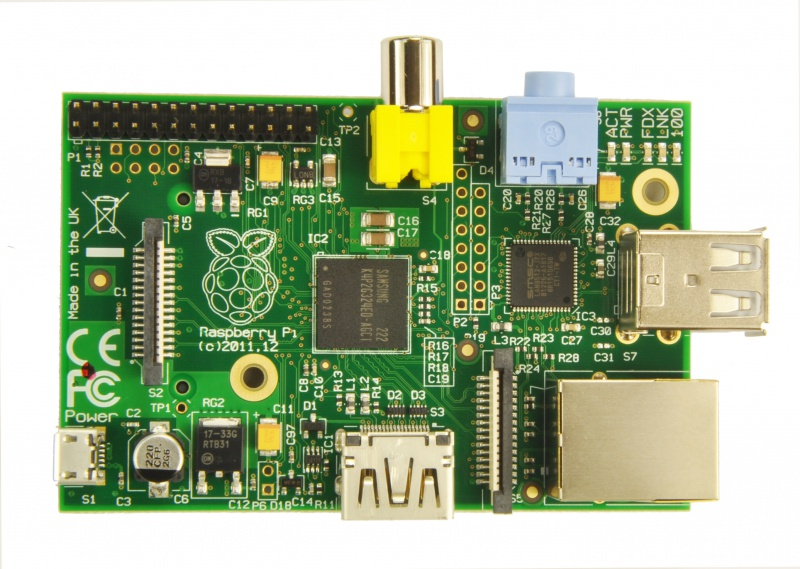
\includegraphics[width=0.5\textwidth]{raspberrypi-front.jpg}
  \caption{Raspberry Pi 1 Model B}
  \label{fig:devboard-raspberrypi}
\end{figure}
% http://elinux.org/File:RpiFront.jpg
% wget http://elinux.org/images/thumb/9/96/RpiFront.jpg/800px-RpiFront.jpg
% mv 800px-RpiFront.jpg raspberrypi-front.jpg


\section{Raspberry Pi 2}

Despite mostly positive reviews for first version of Raspberry Pi, project was also criticized for some hardware design issues.
Fragile SD card dock instead of microSD, electrolytic capacitor used for DC stabilization, wrong USB ports placement and unneeded composite video RCA jack was the most commonly complained.\cite{web:raspberrypi-issues}
Fortunately, all those remarks were taken into consideration and models A+ and B+ were released in 2014 without those drawbacks.
The iconic hardware layout was established, although it was still ``version 1'' without any further innovations, because all of the core parts, including microcontroller, remains the same.

In the 2015, version 2 was released, with the same layout, but new Broadcom BCM2836 SoC.
The most important is that it comes with newer ARMv7-A architecture.
More and more project are being inspired by Raspberry Pi: from its expansions like pi-top modular laptop to imitations like Orange Pi or Banana Pi.\cite{web:pi-top}


\begin{figure}[htbp]
  \centering
    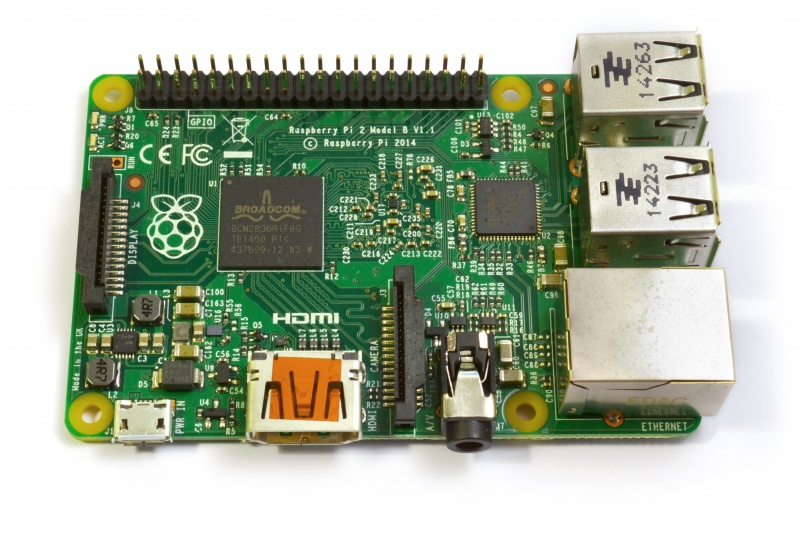
\includegraphics[width=0.5\textwidth]{raspberrypi2-front.jpg}
  \caption{Raspberry Pi 2 Model B}
  \label{fig:devboard-raspberrypi2}
\end{figure}
% https://elinux.org/File:Raspberry_Pi_2_Model_B.jpg
% wget https://elinux.org/images/thumb/7/79/Raspberry_Pi_2_Model_B.jpg/800px-Raspberry_Pi_2_Model_B.jpg
% mv 800px-Raspberry_Pi_2_Model_B.jpg raspberrypi2-front.jpg


% https://pi-top.com/products/pi-top


% pi-top


\section{BeagleBone Black}
% https://beagleboard.org/black

BeagleBone Black, together with preceding BeagleBone (White) and BeagleBoard are often named a competitors for the Raspbery Pi series.
Most important difference is that they are build upon Texas Instrument SoCs.

The ``Black'', that was released in 2013 gains a lot of attention from more advanced users, that were able to see some of its advantage points, especially in comparison to first version of Raspberry Pi.
Most appraisal goes to well placed expansion connectors, standard 5V power jack, MII based Ethernet (not through USB) and 2 GB of eMMC flash memory with pre-installed Angstrom Linux distribution.
From build systems perspective, it is a big plus that TI AM3358 SoC support, is included into Linux kernel mainline, which means that there is no need for special patches.

There are stil more and more boards being developed from this comunity including BeagleBoard X15 (2016), BeagleBone Green, BeagleBoard Blue and competitor to Raspbery Pi Zero: PockerBeagle (2017).

\begin{figure}[htbp]
  \centering
    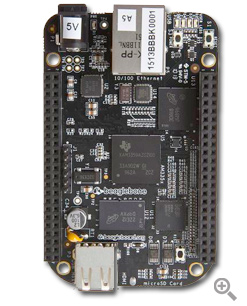
\includegraphics[width=0.25\textwidth]{beaglebone-front.jpg}
  \caption{BeagleBone Black}
  \label{fig:devboard-beaglebone}
\end{figure}
% http://elinux.org/File:BeagleBone-Black-A5_product_detail_black_sm.jpg
% wget http://elinux.org/images/a/ac/BeagleBone-Black-A5_product_detail_black_sm.jpg
% mv BeagleBone-Black-A5_product_detail_black_sm.jpg beaglebone-front.jpg

\section{PandaBoard}
% http://pandaboard.org/

PandaBoard was released in 2010, so it could be called a predecessor of other boards in its class. Despite having very strong ARM Cortex-A9 based TI OMAP4430 chip, that was used also for top class smartphones, everything seems to be very unfortunate.

This board is very large compared to others, and high audio and Ethernet/USB connectors makes it especially unshapely, together with protruding full-size SD card. Ethernet is unfortunately provided just through USB hub chip. RS232 serial DB-9 connector is much less useful, that just making UART pins available, but using totally not popular USB type AB is even more ridiculous. After some initial popularity, most of community has scatted, that is especially painful when dealing with no support for its graphic hardware. The sad last cord happens when the domain \url{pandaboard.org} was not prolonged in 2017 and acquired by bots, which make all links from official documentation unavailable.

\begin{figure}[htbp]
  \centering
    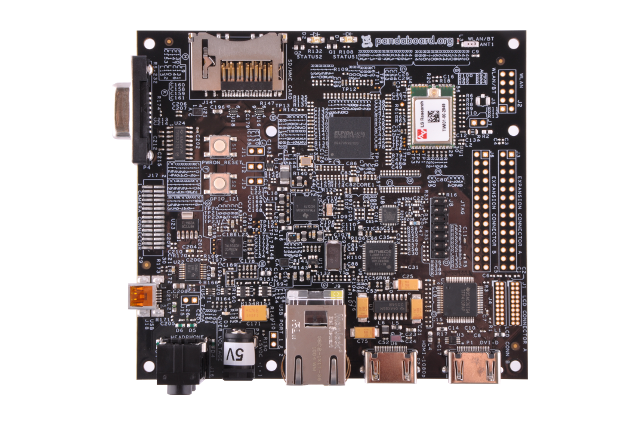
\includegraphics[width=0.5\textwidth]{pandaboard-front.png}
  \caption{Pandaboard}
  \label{fig:devboard-pandaboard}
\end{figure}
% http://elinux.org/File:PandaBoard_front.png
% wget http://elinux.org/images/4/48/PandaBoard_front.png
% mv PandaBoard_front.png pandaboard-front.png





\section{Wandboard Quad}
% https://www.wandboard.org/products/wandboard/WB-IMX6Q-BW/

\begin{figure}[htbp]
  \centering
    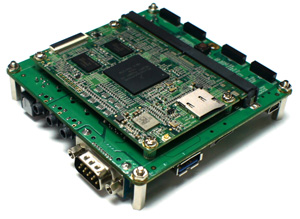
\includegraphics[width=0.5\textwidth]{wandboard-front.jpg}
  \caption{Wandboard}
  \label{fig:devboard-wandboard}
\end{figure}
% http://elinux.org/File:Wandboard-dual.jpg
% wget http://elinux.org/images/7/7b/Wandboard-dual.jpg
% mv Wandboard-dual.jpg wandboard-front.jpg

This board represents the most powerfull i.MX 6 series SoC that was produced by Freescale (currently NXP, but also acquired by Qualcomm).
One of the best advantages from this series, is that there are many types (i.e. Solo, Dual, Quad), that are pin to pin compatible.
That makes it very friendly to mass-scale, but diverse hardware development, so there exists three typed of WandBoard depenting on number of cores.
Many aspects and examples compatible with this board were described in ``Linux w systemach i.MX 6 series'' by Marcin Bis.\cite{book:lws-imx6}


\section{x86\_64 (Asus Eee PC 1215n)}
% https://www.asus.com/Laptops/Eee_PC_1215N/

There is nothing special about this laptop, I choose it mostly because that is the x86\_64 device that I own. Because it is quite old and not aiming to be very powerful, its performance is comparable to development boards, like i.e. Wadnboard Quad. Fortunately it also have a SD card slot, so could be booted in the same way as others.

\begin{figure}[htbp]
  \centering
    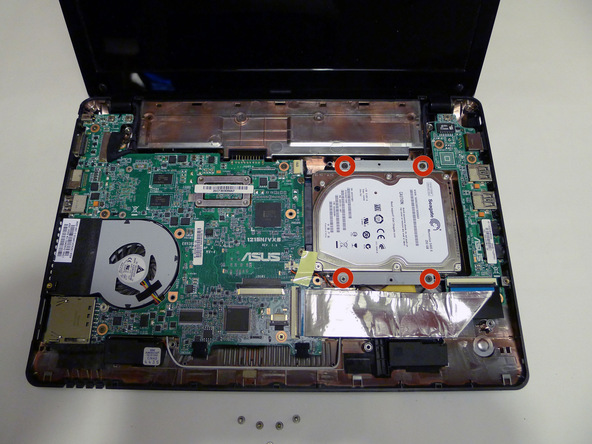
\includegraphics[width=0.5\textwidth]{1215n-front.jpg}
  \caption{Asus Eee PC 1215n}
  \label{fig:devboard-1215n}
\end{figure}
% https://www.ifixit.com/Guide/Asus+Eee+PC+1215N+Hard+Drive+Replacement/12291
% wget https://d3nevzfk7ii3be.cloudfront.net/igi/eKGfAILyYUfWpePd.medium
% mv eKGfAILyYUfWpePd.medium 1215n-front.jpg






%\section{Grinn liteboard}
% http://wiki.litesom.grinn-global.com
% http://linuxgizmos.com/open-spec-sandwich-style-sbc-runs-linux-on-i-mx6ul-based-com/
% wget http://files.linuxgizmos.com/grinn_liteboard.jpg
% mv grinn_liteboard.jpg liteboard-front.jpg
%
%\begin{figure}[htbp]
%  \centering
%    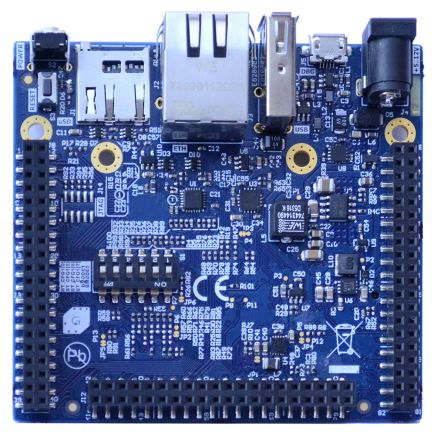
\includegraphics[width=0.5\textwidth]{liteboard-front.jpg}
%  \caption{Liteboard}
%  \label{fig:devboard-liteboard}
%\end{figure}

% Grinn liteboard
% August 2016
% \$120
% 32-bit
% i.MX 6Ultra Light
% ARM Cortex-A7
% 528 MHz
% 512MB DDR3
% 5V & 5V/micro USB
% USB 2.0
% 10/100 half duplex
% 2GB eMMC




\section{Devices comparison}

\begin{landscape}

\renewcommand{\arraystretch}{2}
\begin{table}
  \begin{tabular}{| p{2.5cm} | p{3cm} | p{3cm} | p{3.5cm} | p{3.5cm} | p{3cm} | p{3cm} |}
    \hline
    name & Raspberry Pi 1 & Raspberry Pi 2 & BeagleBone Black & PandaBoard & Wandboard Quad & Asus Eee PC 1215n \\
    \hline
    release date & April 2012 & February 2015 & April 2013 & October 2010 & February 2013 & August 2010\\
    \hline
    target price & \$35 & \$35 & \$45 & \$174 & \$129 & \$499\\
    \hline
    word size & 32-bit & 32-bit & 32-bit & 32-bit & 32-bit & 32-bit/64-bit \\
    \hline
    SoC & Broadcom BCM2835 & Broadcom BCM2836 & Texas Instruments AM3358/9 & Texas Instruments OMAP4430 & Freescale i.MX6 Quad & Intel Atom\\
    \hline
    architecture & ARM Cortex-A7 & ARM Cortex-A8 & ARM Cortex-A8 & ARM Cortex-A9 & ARM Cortex-A9 & x86\\
    \hline
    CPU frequency & 700 MHz & 1000 MHz & 1000 MHz & 1000 MHz & 1000 MHz & 1800 MHz\\
    \hline
    RAM size & 512 GB DDR3 & 1 GB & 512 MiB DDR3 & 1 GB & 2GB DDR3 & 2GB DDR3\\
    \hline
    Power source & 5 V (Micro USB/GPIO) & 5 V (Micro USB/GPIO) & Mini USB / 5 V jack & 5V & 5V & 19V\\ %power consumption?
    \hline
    USB & 2 (via the on-board 5-port USB hub) & 4 (via the on-board 5-port USB hub) & USB 2.0 & two USB host ports and one USB On-The-Go & USB 3.0 & USB 2.0 + USB 3.0\\
    \hline
    Network & 10/100 Mbit/s Ethernet on the USB hub & 10/100 Mbit/s Ethernet on the USB hub  & Ethernet Fast Ethernet (MII based) & 10/100 Ethernet on USB hub & GbE & 10/100 Ethernet (MII based)\\
    \hline
    storage & MicroSDHC slot & MicroSDHC slot & 4GB eMMC / MicroSDHC slot & SDHC slot & MicroSDHC & SATA (default 320 GB HDD)\\
    \hline
  \end{tabular}
  \caption{Development boards comparison}
\end{table}

\end{landscape}



















\chapter{Linux build systems for embedded devices}
\label{chapter:build-systems}
%\section{Creating a basic Linux system}
%\label{section:basic-system}






In this chapter I will describe all embedded Linux build systems in order of rising complexity.
Since there is nothing more practical than a good example, the list of all shell commands that are essential to run complete build process, is presented on the beginning of each section.
It will be then discussed line by line, in a reference to OS build systems structure presented in Section \ref{section:builders-structure}.
Suggested way is not to copy and paste entire script, but rather execute commands line by line.
In some cases input from user is needed, what will be marked with commented lines (using \#).

To run freshly created distribution on Raspberry Pi from SD card in smallest possible number of steps is for distribution builders something like like printing ``Hello world!'' for programming or ``blinking a led'' for electronics project.
The most generic way seems to be just using Host OS as Target OS, but it excludes cross-compilation and testing system on real embedded device.

Each of the examples assumes, that it is executed on freshly installed Debian instance.
To get prerequisites for all builders installed at once, following command could be executed:


\begin{lstlisting}
sudo apt install make gcc g++ libncurses-dev unzip git \
  patch python python-dev rsync bc bzip2 gawk zlib1g-dev \ 
  bison flex tcl gettext lzop gawk diffstat texinfo \
  build-essential chrpath pkg-config pv
\end{lstlisting}

At the end of each script, the final image is being copied to home directory, to highlight its location.
It could be especially useful when running build on special server and then downloading it to local machine in order to deploy it on real SD card.
It could be done in many ways, even on Windows systems, but below I present the one that is most convinient for me:

\begin{lstlisting}
pv sdcard.img | sudo dd of=/dev/sdb bs=4M oflag=dsync
\end{lstlisting}

With the use of \verb|pv| tool, the progress of mission-critical \verb|dd| could be monitored. Here, \verb|/dev/sdb| is just most common example of SD card device, but each time it should be checked.








% ----------------------------------------------------------------
% ----------------------------------------------------------------
% ----------------------------------------------------------------
% ----------------------------------------------------------------




\section{Buildroot}
% https://www.slideshare.net/tpetazzoni/buildroot-building-embedded-linux-systems-made-easy-linux-conf-australia-2014
% https://events.linuxfoundation.org/sites/events/files/slides/belloni-petazzoni-buildroot-oe_0.pdf
% http://linuxgizmos.com/free-embedded-linux-training-materials-demystify-buildroot/


\begin{figure}[htbp]
  \centering
    
\includegraphics[width=0.5\textwidth]{buildroot-logo.png}
    \caption{Buildroot logo}
  \label{fig:buildroot-logo}
\end{figure}
%https://buildroot.org/images/logo.png

Buildroot is named a simple, efficient and easy-to-use tool to generate embedded Linux systems through cross-compilation. The name came from the process of building the root filesystem.

It's initial public release takes place at January 2005. Latest stable release is 2017.11.1. The project is backed by the group of open source developers, not directly by any organization, but gets financial sponsorship from various companies. Especially the involvement of Thomas Petazzoni, the Chief Technical Officer of Free Electrons is worth to notice.\cite{web:buildroot-tpetazzoni}

%  The only difference between boards is \verb|defconfig| name.

% TODO: add other packages, i.e. for buildroot - patch python rsync bc bzip2 (bzcat)
\begin{lstlisting}
sudo apt install make gcc g++ libncurses-dev unzip git 

wget https://buildroot.org/downloads/buildroot-2017.11.1.tar.bz2
tar -xjf buildroot-2017.11.1.tar.bz2
cd buildroot-2017.11.1/

export MACHINE=raspberrypi

make raspberrypi_defconfig
time make
cp output/images/sdcard.img ~
\end{lstlisting}



\subsection*{Source code}

Buildroot is the simplest among build systems from every point of view.
Its source code releases could be downloaded from main website in two popular archive formats: tar.bz2 and tar.gz.
The example of downloading is shown in line number 3.
Source code that do not belong into buildroot core is downloaded during build process.

\subsection*{Host OS requirements}

This initial package requirements for host OS, visible in line 1, are the smallest among all build systems.
They seems to be obvious, but because they are only a few, each could be described:

\begin{itemize}
    \item \verb|make| - the main build utility, that run commands specified in \verb|Makefile|s
    \item \verb|gcc|, \verb|g++| - C and C++ compilers, that will create a specyfic cross-compilation toolchain
    \item \verb|libncurses-dev| - library that makes able to create \verb|menuconfig| GUI in terminal
    \item \verb|unzip|, \verb|git| - most basic tools to getting source code and unpack archives
\end{itemize}

\subsection*{Cross-compilation toolchain}

The buildroot toolchain is based on GCC and could be compiled with use of various C libraries, like uClibc-ng, glibc and musl. It is possible to use buildroot only for its creation, so that it could compile stand alone project or included as part of another builder. To achieve that, just command \verb|make toolchain| need to be invoked.

\subsection*{Target OS configuration}

As mentioned before, configuration management is borrowed from Linux kernel.
\verb|make menuconfig| will open terminal GUI and results could be saved in \verb|.config| file.
It is very convenient to just put that file under version control of target embedded project.
There is also a lot of base configurations, that could be listed with \verb|make list-defconfig| and applied as shown in line 9.
The configuration of Linux kernel could be accessed via \verb|make linux-menuconfig|

\subsection*{Produced output}
The login prompt on embedded device is shown on picture below.
It is a tradition that default and only available admin user is \verb|root| with empty password.
Of course it could stay that way only for development purposes.

\begin{figure}
    \centering
\begin{verbatim}
Welcome to Buildroot
buildroot login: root
# uname -a
Linux buildroot 4.9.52 #1 Sat Wed 24 12:00:00 UTC 2018 armv6l GNU/Linux
\end{verbatim}
    \caption{buildroot - raspberrypi}
\end{figure}












% ----------------------------------------------------------------
% ----------------------------------------------------------------
% ----------------------------------------------------------------
% ----------------------------------------------------------------




\section{OpenWRT}
% http://events17.linuxfoundation.org/sites/events/files/slides/ELC_OpenWrt_LEDE.pdf
% https://wiki.openwrt.org/toh/raspberry_pi_foundation/raspberry_pi
% https://lede-project.org/toh/hwdata/raspberrypifoundation/raspberrypifoundation_raspberrypi_bplus
% https://lede-project.org/docs/guide-developer/quickstart-build-images
% https://lede-project.org/docs/guide-developer/compile_packages_for_lede_with_the_sdk

\begin{figure}[htbp]
  \centering
    
\includegraphics[width=0.5\textwidth]{openwrt-logo.png}
    \caption{OpenWrt logo}
  \label{fig:openwrt-logo}
\end{figure}
%https://openwrt.org/.styles/img/openwrt-logo.png

OpenWrt is named a Linux distribution for embedded devices. The name came from open source firmware for WRT54G series of wireless routers.

It's initial public release takes place at January 2004. In May 2016 a group of its core developers decided to fork the project and create LEDE - Linux Embedded Development Environment. Fortunately in January 2018, it was officially announced that both projects will merge under the ``OpenWrt'' branding.





\begin{lstlisting}
sudo apt install make gcc g++ libncurses-dev unzip git gawk file zlib1g-dev
git clone -b v17.01.4 https://github.com/openwrt/openwrt
cd openwrt/
./scripts/feeds update -a
./scripts/feeds install -a
make defconfig
make menuconfig
# Target System (Broadcom BCM27xx)
# Target Profile (Raspberry Pi B/B+/CM/Zero/ZeroW)
time make
cp build_dir/target-arm_arm1176jzf-s+vfp_musl-1.1.16_eabi/linux-brcm2708_bcm2708/tmp/lede-brcm2708-bcm2708-rpi-ext4-sdcard.img ~
\end{lstlisting}



\subsection*{Source code}

To get specific version of OpenWrt code one should get it thought git SCM, eventually pointing to a specific version tag.
Significantly, that from the beginning of 2018, merged source code is available from OpenWrt repository, but in some places still LEDE brand could be seen.
It is specific for this system, that there is also a need to update and install package definitions, as shown in lines 4 and 5

\subsection*{Host OS requirements}

Package preliminary requirements are just a little bigger than in Buildroot.

\subsection*{Cross-compilation toolchain}

Since OpenWrt is a Buildroot-based fork, there is also a possibility to create only toolchain in a very similar way: \verb|make toolchain/install|.

\subsection*{Target OS configuration}

Unfortunately, in this build system it is not possible to choose one of available base configurations from command line, so it need to be selected from menuconfig ncurses-based GUI.
As OprnWrt puts primary focus on routers and other networking devices, it is strongly visible in great availability of related packages.

\subsection*{Produced output}

Login prompt could be seen on included figure.
LEDE logo is still shown, as a result of ongoing merge process.


\begin{figure}
    \centering
\begin{verbatim}
BusyBox v1.25.1 () built-in shell (ash)

     _________
    /        /\      _    ___ ___  ___
   /  LE    /  \    | |  | __|   \| __|
  /    DE  /    \   | |__| _|| |) | _|
 /________/  LE  \  |____|___|___/|___|                      lede-project.org
 \        \   DE /
  \    LE  \    /  -----------------------------------------------------------
   \  DE    \  /    Reboot (17.01.4, r3560-79f57e422d)
    \________\/    -----------------------------------------------------------

=== WARNING! =====================================
There is no root password defined on this device!
Use the "passwd" command to set up a new password
in order to prevent unauthorized SSH logins.
--------------------------------------------------
root@LEDE:/# uname -a
Linux LEDE 4.4.92 #0 Wed Oct 24 12:00:00 2017 armv6l GNU/Linux
\end{verbatim}
    \caption{openwrt - raspberrypi}
\end{figure}






% ----------------------------------------------------------------
% ----------------------------------------------------------------
% ----------------------------------------------------------------
% ----------------------------------------------------------------



\section{LTIB}
% http://ltib.org/home-intro 
% http://ltib.org/pages/LTIB_generic_v1.4_-_version_6.4.1.pdf
% http://www.bitshrine.org/autodocs/LtibFaq.html#ref_10
% What is required on your host before installing LTIB



\begin{figure}[htbp]
  \centering
    
\includegraphics[width=0.1\textwidth]{ltib-logo.png}
    \caption{LTIB logo}
  \label{fig:ltib-logo}
\end{figure}
%http://ltib.org/graphics/ltib_logo32.png


\begin{figure}[htbp]
  \centering
    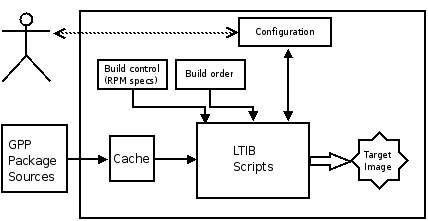
\includegraphics[width=\textwidth]{ltib-diagram.png}
    \caption{LTIB structure diagram}
  \label{fig:ltib-diagram}
\end{figure}
%http://ltib.org/graphics/ltib_build.png


LTIB is officially called a tool that can be used to develop and deploy BSPs (Board Support Packages) for a number of embedded target platforms. The name came from Linux Target Image Builder.

It was launched and financed by Freescale Seminconductor around 2004-2005. In 2009 project was transferred to Savannah, but its development stopped at 2013 with version 13.2.1.


% echo "cdynak ALL = NOPASSWD: /usr/bin/rpm, /opt/ltib/usr/bin/rpm" >> /etc/sudoers


% https://midnightyell.wordpress.com
% https://github.com/midnightyell/RPi-LTIB
% rpm -ivh ... (missing ltib rpi tools)
% http://nongnu.13855.n7.nabble.com/Raspberrypi-toolchain-is-missing-from-gpp-td78878.html

% bash "No such file or directory" (32 / 64 bit...)
% https://askubuntu.com/questions/133389/no-such-file-or-directory-but-the-file-exists
% sudo dpkg --add-architecture i386 , etc...
% debian install 32 bit libz
% 64-bit Debian or Ubuntu : apt-get install zlib1g:i386

% ti_3410.fw ltib
% https://github.com/raspberrypi/linux/issues/112
% https://github.com/raspberrypi/linux/commit/e6ef7f6bbc05fdcd7b1f115bb55a32c176663296
% apply patch... for arch/arm/mach-bcm2708/bcm2708.c and drivers/usb/host/dwc_otg/dwc_otg_driver.c
% rpm/BUILD/raspberrypi-linux-118e2d3/arch/arm/mach-bcm2708/bcm2708.c
% rpm/BUILD/raspberrypi-linux-118e2d3/drivers/usb/host/dwc_otg/dwc_otg_driver.c

% on ubuntu 14.04 32 bit...
% https://stackoverflow.com/questions/25438455/ltib-installation-woes
% http://nongnu.13855.n7.nabble.com/Linux-Mint-1-6-Can-t-get-rpm-4-0-4-tar-gz-at-ltib-line-834-td75924.html
% http://ftp.rpm.org/releases/historical/rpm-4.0.x/rpm-4.0.4.tar.gz

% /sbin/fdisk -l output/images/sdcard.img
% no bootable flag/not working...
% "wrong fs type, bad option, bad superblock"
% mount sdcard image locally ...
% https://askubuntu.com/questions/445979/how-to-mount-sd-card-image-created-with-dd
% https://en.wikibooks.org/wiki/QEMU/Images#Mounting_an_image_on_the_host

\begin{lstlisting}
sudo apt install make gcc g++ libncurses-dev unzip rpm bison patch tcl zlib1g-dev

wget https://github.com/downloads/midnightyell/RPi-LTIB/raspberrypi-tools-9c3d7b6-1.i386.rpm
sudo mkdir -p /opt/ltib/pkgs/
sudo cp raspberrypi-tools-9c3d7b6-1.i386.rpm /opt/ltib/pkgs/

sudo dpkg --add-architecture i386
sudo apt update
sudo apt install zlib1g:i386 libstdc++:i386

wget http://download.savannah.nongnu.org/releases/ltib/ltib-13-2-1-sv.tar.gz
tar -xzf ltib-13-2-1-sv.tar.gz
cd ltib-13-2-1-sv/
time ./ltib

# Platform choice (Raspberry Pi with BCM2835 SoC)

cp output/images/sdcard.img ~
\end{lstlisting}




\subsection*{Source code}

Since LTIB development was moved to Savannah, it is possible to obtain tar.gz compiled code throught HTTP from there, as shown in line 13.
Source code was maintained with the use of archaic cvs SCM, which shows how long time ago it was initiated.
In relation to source code, it is also worth to mention, that \verb|./ltib| which is the initiating bash script, have 3000+ lines of code which for sure made it hard to maintain. 

\subsection*{Host OS requirements}

Host requirements are more and more intricate, due to halted LTIB development and rapid development of host systems, like Debian.
There is a need to add i386 architecture support on host OS (line 7) and then install necessary packages (line 9)

\subsection*{Cross-compilation toolchain}

What differs it from previously described systems, is that cross-compilation toolchain is installed globally.
Because of that, there is a need to have administrative privileges, most preferably just \verb|sudo| permissions.
Some of platform (Raspberry Pi) specific packages are missing and they need to be prepared separately, as described in lines 3-5.

\subsection*{Target OS configuration}

Here configuration is also based on \verb|menconfig|.
The step with choosing platform need to be performed manually, in the way that is commented on line 16.
% ./ltib -m imx6q ?

\subsection*{Produced output}

Unfortunately this build system is so old, that it could support only first version of Raspberry Pi and no other from presented development boards.

% ----------------------------------------------------------------
% ----------------------------------------------------------------
% ----------------------------------------------------------------
% ----------------------------------------------------------------




\section{PTXdist}

% http://elinux.org/PTXdist
% http://public.pengutronix.de/oselas/bsp/pengutronix/OSELAS.BSP-Pengutronix-Generic-arm-Quickstart.pdf
% http://public.pengutronix.de/oselas/toolchain/
% http://public.pengutronix.de/software/ptxdist/
% http://public.pengutronix.de/software/ptxdist/appnotes/
% https://git.pengutronix.de/cgit/DistroKit
% https://www.pengutronix.de/en/2017-08-28-distrokit-a-playground-bsp-for-ptxdist.html
% https://ptxdist.org/doc/user_manual_section.html

% https://www.mail-archive.com/ptxdist@pengutronix.de/msg10260.html
% Difference between DIstroKit and OSELAS.BSP-Pengutronix-Generic



\begin{figure}[htbp]
  \centering
    
\includegraphics[width=0.75\textwidth]{ptxdist-logo.png}
    \caption{PTXdist logo}
  \label{fig:ptxdist-logo}
\end{figure}
%https://www.ptxdist.org/images/PTXdist_Logo_RGB.svg
%https://www.rauc.io/images/ptxdist_logo.png

PTXdist is called a build system that creates embedded Linux distributions directly from the source code. The name came from combining shortcut of company Pengutronix and and word ``distribution''.

Its initial public release dates back to 2010 and the latest stable version is 2017.12.0. Its developed and maintained by the German company Pengutronix.



\subsection*{Basic system}
% https://debian.pkgs.org/sid/rt-preempt-nonfree-i386/oselas.toolchain-2013.12.1-arm-1136jfs-linux-gnueabihf-gcc-4.8.2-glibc-2.18-binutils-2.24-kernel-3.12-sanitized_2013.12.1_i386.deb.html
% https://debian.pkgs.org/sid/rt-preempt-nonfree-i386/oselas.toolchain-2016.06.0-arm-1136jfs-linux-gnueabihf-gcc-5.4.0-glibc-2.23-binutils-2.26-kernel-4.6-sanitized_2016.06.0_.deb.html

% only when building all with ./build_all_v2.mk
% http://ptxdist.pengutronix.narkive.com/iZ6AhfNp/pull-request-oselas-toolchain-for-upstream-update-for-gcc-4-4-1-and-binutils-2-20
% ln -s /usr/local/bin/ptxdist p

% http://www.friendlyarm.net/forum/topic/4535 (OSELAS Toolchain)

% (missing) lzop barebox



% # sudo mkdir -p /opt/OSELAS.Toolchain-2016.06.1/
% # sudo chown debian:debian /opt/OSELAS.Toolchain-2016.06.1/
% # time ptxdist go

% wget http://debian.pengutronix.de/debian/pool/main/o/oselas.toolchain/oselas.toolchain-2016.06.1-arm-1136jfs-linux-gnueabihf-gcc-5.4.0-glibc-2.23-binutils-2.26-kernel-4.6-sanitized_2016.06.1_amd64.deb
% sudo dpkg -i oselas.toolchain-2016.06.1-arm-1136jfs-linux-gnueabihf-gcc-5.4.0-glibc-2.23-binutils-2.26-kernel-4.6-sanitized_2016.06.1_amd64.deb


\begin{lstlisting}
sudo apt install make gcc g++ libncurses-dev unzip git gawk flex bison gettext python-dev lzop pkg-config libxml-parser-perl

wget http://public.pengutronix.de/software/ptxdist/ptxdist-2018.01.0.tar.bz2
tar -xjf ptxdist-2018.01.0.tar.bz2
cd ptxdist-2018.01.0
./configure
make
sudo make install
cd ..

wget http://public.pengutronix.de/software/ptxdist/ptxdist-2016.06.0.tar.bz2
tar -xjf ptxdist-2016.06.0.tar.bz2
cd ptxdist-2016.06.0
./configure
make
sudo make install
cd ..

wget https://public.pengutronix.de/oselas/toolchain/OSELAS.Toolchain-2016.06.1.tar.bz2
tar -xjf OSELAS.Toolchain-2016.06.1.tar.bz2
cd OSELAS.Toolchain-2016.06.1/
ptxdist-2016.06.0 select ptxconfigs/arm-1136jfs-linux-gnueabihf_gcc-5.4.0_glibc-2.23_binutils-2.26_kernel-4.6-sanitized.ptxconfig
ptxdist-2016.06.0 migrate
time ptxdist-2016.06.0 go

git clone https://git.pengutronix.de/cgit/DistroKit/
cd DistroKit/
ptxdist-2018.01.0 platform configs/platform-rpi/platformconfig
ptxdist-2018.01.0 migrate
time ptxdist-2018.01.0 images
cp platform-rpi/images/hd.img ~
\end{lstlisting}

% for rpi2 and beaglebone
% ptxdist-2016.06.0 select ptxconfigs/arm-v7a-linux-gnueabihf_gcc-5.4.0_glibc-2.23_binutils-2.26_kernel-4.6-sanitized.ptxconfig
% ptxdist-2018.01.0 platform configs/platform-v7a/platformconfig
% cp platform-v7a/images/*hdimg* ~



\subsection*{Source code}

For this build system it is not possible to download all its sources, because it is split into 3 parts:

\begin{itemize}
    \item PTXdist - specific higher level (than i.e. make) build tool, aimed to ``execute documentation''
    \item OSELAS.Toolchain - toolchain suggested by PTXdist
    \item DistroKit - named a Build Support Package example, it is where default configurations for platforms like i.e. Raspbery Pi came from
\end{itemize}

\subsection*{Host OS requirements}

There is nothing specific about hot OS requirements, beside that it is written explicitly in documentation, that there is a need to install globally two versions of PTXdist (lines 3-17).
Latest one will be used for all operations, with the exception for building cross-compilation toolchain, for which the older one is needed.

\subsection*{Cross-compilation toolchain}

The OSELAS.Toolchain has not been updated since 2016 and that is why compatible ptxdist-2016.06.0 is needed.
There is also a need to make an arbitrary decision about target cross compilation architecture, because it will be installed globally before configuring target.
Example for Raspberry Pi is shown in lines 19-25.
To create one for each architecture at once the script \verb|./build_all_v2.mk| could be run, but since there are about 16 different, it will take enormous amount of time.
It is also possible to use binary packages of those toolchain, what is available to download from Pengutronix website.

\subsection*{Target OS configuration}

PTXdist command line tool could be used to create so called BSP for any platform, but configurations for popular development boards are available in DistroKit.
For every other build system ``u-boot'' is chosen as default bootloader, but here it is the ``barebox'', which is being developed by Pengutronix company.

\subsection*{Produced output}

For ARMv7 devices, target configuration it grouped under \verb|platform-v7a|, so final distinction for building SD card image is made upon device tree file.


% ----------------------------------------------------------------
% ----------------------------------------------------------------
% ----------------------------------------------------------------
% ----------------------------------------------------------------



\section{Yocto Project}

\begin{figure}[htbp]
  \centering
    
\includegraphics[width=0.75\textwidth]{yoctoproject-logo.png}
    \caption{Yocto Project logo}
  \label{fig:yoctoproject-logo}
\end{figure}
% http://www.yoctoproject.org/docs/current/yocto-project-qs/figures/yocto-project-transp.png

The Yocto Project is named an open source collaboration project that provides templates, tools and methods to help you create custom Linux-based systems for embedded products. Its name came from the smallest metric system unit prefix ``yocto'' that emphasize possibility to create tiny distributions.

The project under it's current name was formed in 2010-2011 and the latest stable version is 2.4 ``Rocko'' released at October 2017. The Yocto Project is a lab workgroup of the Linux Foundation and its developed and maintained by the group of major companies, including ...







\begin{lstlisting}
wget http://commondatastorage.googleapis.com/git-repo-downloads/repo
chmod a+x repo
sudo mv repo /usr/local/bin/

sudo apt install make gcc g++ unzip git
sudo apt install gawk diffstat texinfo build-essential chrpath

export MACHINE=raspberrypi

mkdir yoctoproject
cd yoctoproject
repo init -u https://github.com/cdynak/yocto-manifest -m $MACHINE.xml
repo sync

source poky/oe-init-build-env
MACHINE=wandboard DISTRO=poky source setup-environment build
% vi conf/bblayers.conf (...?)
time bitbake core-image-minimal
cp tmp/deploy/images/$MACHINE/*img ~
\end{lstlisting}


\subsection*{Source code}

The source code structure of Yoctro Project could be named the most complex, because it introduced concept of layers.
They are divided into several groups:
\begin{itemize}
    \item Base - there are only two core layers: \verb|openembedded-core| and \verb|meta-oe|, which need to be included for all projects
    \item Machine (BSP) - responsibility certain platforms support is split in this group, i.e. ``meta-ti'' layer provide configuration for both BeagleBone and PandaBoard and it is maintained with the help of Texas Instruments company
    \item Software - specific pieces of software are divided into layers like ``meta-nodejs'' for nodejs and ``meta-ros'' for Robotic Operating System packages
    \item Distribution - 
    \item Miscealous - the rest, that do not fit into any other group, i.e. when it could be clasified for more than one group
\end{itemize}

\subsection*{Host OS requirements}

There is a need to have only basic packages on host operating systems, because everything else will be created in local directory as needed.
Specific exception could be a ``repo'' tool, which installation is made in lines 1-3.
It was borrowed from Android project, because it helps in to download multiple git repositories, based on provided XML configuration file.
Layers could be downloaded and configured manually, but most of Yocto Project developer guides suggests to use this tool.

\subsection*{Cross-compilation toolchain}
It is also possible to only create a toolchain with command \verb|bitbake meta-toolchain|.

\subsection*{Target OS configuration}
Target configuration is something what makes this tool very different from the others.
It abandons the ``Makefiles'' executed by ``make'', in favor to ``recepies'' executed by python tool ``bitbake''.
This concept comes from time before Yocto Project was formed and there exists only OpenEmbedded project, which was not aimed to provide easy support for all groups of layers.
Because of its well known complexity, but also flexibility, it reshapes common understanding of ``distribution'' therm, i.e. popular Angstrom Linux distribution is represented by ``meta-angstrom'' and this is how it is being created for x86\_64 targets.

\subsection*{Produced output}
The login prompt on embedded device is shown on picture below.


\begin{figure}
    \centering
\begin{verbatim}
Poky (Yocto Project Reference Distro) 2.2.3 raspberrypi /dev/ttyAMA0
raspberrypi login: root
root@raspberrypi:~# uname -a
Linux raspberrypi 4.4.50 #1 Wed Jan 24 12:00:00 UTC 2018 armv6l GNU/Linux
\end{verbatim}
    \caption{yoctoproject - raspberrypi}
\end{figure}





% ----------------------------------------------------------------
% ----------------------------------------------------------------
% ----------------------------------------------------------------
% ----------------------------------------------------------------


\section{CLFS}

\begin{figure}[htbp]
  \centering
    
\includegraphics[width=0.75\textwidth]{lfs-logo.png}
    \caption{Linux From Scratch logo}
  \label{fig:lfs-logo}
\end{figure}
%http://www.linuxfromscratch.org/images/lfs-logo.png

% http://www.linuxfromscratch.org
% http://trac.clfs.org}
% http://intestinate.com/pilfs/
% https://raspberrypi.stackexchange.com/questions/25/is-there-a-linux-from-scratch-lfs-arm-equivalent

In the begining, there was just LFS project that provides step-by-step instructions for building your own custom Linux system, entirely from source code.
Its name came from Linux From Scratch.
Its initial release was made in December 1999 and its latest stable version is 8.1 from September 2017. The project was initiated by Gerard Beekmans and gains support from many open source enthusiasts.

Then this project grows, the few sub-projects appeared, like Beyond LFS, to instruct future maintaining of custom distribution, as well as Cross LFS.
LFS is well maintained and often have an official release, but CLFS have no regularity in that regard and no useful automation process, so it could be treated rather as a source of tips and tricks, than a build system.

It is also possible to i.e. build new system from within Raspberry Pi using LFS instructions, but it then would not include the essential cross-compilation process.


% ----------------------------------------------------------------
% ----------------------------------------------------------------
% ----------------------------------------------------------------
% ----------------------------------------------------------------


% \section{Distribution custom systems}

% \subsection*{Multistrap}


% ----------------------------------------------------------------
% ----------------------------------------------------------------
% ----------------------------------------------------------------
% ----------------------------------------------------------------


% \section{Non-free and closed Source}

% Horrible, awkward situation - like you need to call a special service to fix your hammer, instead of making it yourself.
% There is a lot of companies, that provides commercial support like: free-electrons, ...

% \subsection*{Wind River Linux}

% ----------------------------------------------------------------
% ----------------------------------------------------------------
% ----------------------------------------------------------------
% ----------------------------------------------------------------




\begin{landscape}

\begin{table}
  \begin{tabular}{| p{3cm} | p{3cm} | p{3cm} | p{3cm} | p{3cm} | p{3cm} | p{3cm} |}
    \hline
    name & Buildroot & OpenWrt & LTIB & PTXdist & Yocto Project & CLFS \\
    \hline
    official website & \url{https://buildroot.org} & \url{https://openwrt.org} & \url{http://ltib.org} & \url{https://ptxdist.org} & \url{https://yoctoproject.org} & \url{http://clfs.org}\\
    \hline
    last stable release date & 2017.11 & 2017.01 & 2013.02 & 2018.01 & 2017.10 & 2014.10\\
    \hline
    release cycle & three month\cite{web:buildroot-releases} & irregular (approx 1 year) & irregular (approx 2 years)\cite{web:ltib-releases} & one month\cite{web:ptxdist-releases} & six months\cite{web:yoctoproject-releases} & irregular\cite{web:clfs-releases}\\
    \hline
    number of supported packages &  &  &  &  &  & \\
    \hline
    number of supported boards &  &  &  &  &  & \\
    \hline
    total number of required packages &  &  &  &  &  & \\
    \hline
    total size of required packages &  &  &  &  &  & \\
    \hline
    name &  &  &  &  &  & \\
    \hline
  \end{tabular}
  \caption{Embedded Linux build systems overview}
\end{table}



% maybe make it available to download .config file from os.builders ...?

% google trends ...?

% git repo path (for every system)

% license

% https://www.yoctoproject.org/toaster/all-machines.html
% http://layers.openembedded.org/layerindex/branch/master/machines
% http://www.bitshrine.org/autodocs/bsp_ext_ava.html
% buildroot -> make list-defconfigs | grep ... (defconfig?) | wc -l




% required packages - on freshly installed debian system


% TODO: table
% official repository / github mirror / download directory
% repository links / vcs - table / comparison ...
% os requirements / packages + hardware requirements + download rates! + google analitics popularity! + how did they name themselves... + nr of packages available + main site + documentation site
% notes about release process / release cycles / frequency?






% WARNING: DEGRADATION OF SD CARDS! (ram file system... and other mechanisms)

% vi board/grinn/liteboard/genimage.cfg
% rm output/images/*
% make uboot-rebuild
% make linux-rebuild
% make


% bare debian missing packages...: file

% finish the builder/device matrix table with config names

% compare how many 



\end{landscape}



















\chapter{Build process comparison}
\label{chapter:build-comparison}

\section{Build servers}
In Chapter \ref{chapter:build-systems}, only the software requirements for each build system were specified, but because of enormous amount of compilation happening, hardware resources are significant.
Even if local PC or laptop have have very good parameters, it is very hard to provide at home Internet connection with constant bandwidth, which is important to compare time of each build process, because all package sources are being downloaded meanwhile.
To have isolated environment with guaranteed parameters it is reasonable to use external hosting service.

I choose OVH, because it is the one, that I am used to, especially I enjoy user interface, which is even open sources at \url{https://github.com/ovh-ux/ovh-manager-web}.
More reasonable arguments in favor to OVH is that it have datacenter in Poland (WAW) and enables direc access to OpenStack interface.
For measure basic compilation time for each board and system respectively I use dedicated server, which is the most efficient option.
Nevertheless, I also made tests with virtual machines through OpenStack, because it is very easy to change their parameters and compare growing build time.
Initially, I used ``serwery.pl'' (subsidiary of ``nazwa.pl'' / NetArt) which also provides OpenStack platform, but it was removed in the middle of 2017.


\section{OpenStack configuration}

Before instructions for building target OS, presented in Chapter \ref{chapter:build-systems}, could be executed, there is a need to create and provision virtual machine.

% https://github.com/pkgcloud/pkgcloud
% https://www.alibabacloud.com/
% http://kb.arubacloud.com/en/computing/creating-and-configuring-a-cloud-server/partitioning-and-formatting-an-added-hard-drive-linux-debian.aspx


% m1.tiny - VCPUs: 1, RAM: 512 MB
% m1.2xlarge - VCPUs: 12, RAM: 16,384 MB

% s1-2 - VCPUs: 1, RAM: 2,000 MB
% b2-30-flex - VCPUs: 8, RAM: 29.3 GB / 30,000 MB

\subsection*{VM creation}

\begin{enumerate}
  \item Login to Horizon panel (https://horizon.cloud.ovh.net)
  \item Select ``instances'' and ``launch instance''
  \item Choose instance name (build-server), type (c2-30-flex), image (Debian 9)
  \item Choose or create key pair
  \item Launch instance
  \item Select ``volumes'' and ``create volume'' or... just select ``Boot from image (creates a new volume)'' 
  \item Choose volume name (build-volume), type (SAS), size (50 GB)
  \item Create volume
  \item Attach volume to instance
\end{enumerate}

\subsection{VM provisioning}

\begin{enumerate}
  \item identify (\verb|$HOST_KEYS $HOST_USER $HOST_IP $VOLUME_ID|)
  \item Login with (\verb|ssh -i $HOST_KEYS $HOST_USER@$HOST_IP|)
  \item Update system (\verb|sudo apt update && sudo apt upgrade|)
  \item Create partition on volume (\verb|sudo mkfs.ext4 /dev/sdb|)
  \item Mount volume (\verb|sudo mount /dev/sdb /mnt/|)
  \item (\verb|sudo chown debian:debian /mnt/|)
  \item Navigate to mounted directory (\verb|cd /mnt/|)
\end{enumerate}

\section{Tests in respect to host OS}

\begin{landscape}



\begin{table}
  \begin{tabular}{| p{2.5cm} | p{3cm} | p{3cm} | p{3cm} | p{3cm} | p{3cm} | p{3cm} |}
    \hline
    name & Raspberry Pi 1 & Raspberry Pi 2 & BeagleBone Black & PandaBoard & Wandboard Quad & Asus Eee PC 1215n \\
    \hline
    real time & 17m33.619s & 20m15.836s & 26m12.604s & 11m41.240s & 11m39.519s &  \\
    \hline
    user time & 73m47.968s & 74m30.368s & 55m52.408s & 49m39.200s & 48m33.172s &  \\
    \hline
    sys time & 3m54.620s & 3m58.084s & 3m13.860s & 2m31.172s & 2m27.688s &  \\
    \hline
    buildroot-2017.11.1/ & 5.4G & 5.4G & 6.0G & 4.8G & 4.7G & \\
    \hline
    sdcard.img & 93M & 93M & 77M & 69M & 61M & \\
    \hline
    boot time & 4.926830 & 5.575466 & & ... & 3.640106 & \\
    \hline
  \end{tabular}
  \caption{Buildroot build comparison}
\end{table}


\begin{table}
  \begin{tabular}{| p{2.5cm} | p{3cm} | p{3cm} | p{3cm} | p{3cm} | p{3cm} | p{3cm} |}
    \hline
    name & Raspberry Pi 1 (make) & Raspberry Pi 2 & BeagleBone Black & PandaBoard & Wandboard Quad (make -j) & Asus Eee PC 1215n \\
    \hline
    real time & 47m49.305s &  &  &  & 31m32.177s &  \\
    \hline
    user time & 36m41.768s &  &  &  & 43m14.808s &  \\
    \hline
    sys time & 2m14.996s &  &  &  & 2m33.428s &  \\
    \hline
    openwrt/ & 8.4G &  &  &  & 8.1G &  \\
    \hline
    sdcard.img & 285M &  &  &  &  &  \\
    \hline
    boot time & 8.492709 &  &  &  &  &  \\
    \hline
  \end{tabular}
  \caption{OpenWrt build comparison}
\end{table}




\begin{table}
  \begin{tabular}{| p{2.5cm} | p{3cm} | p{3cm} | p{3cm} | p{3cm} | p{3cm} | p{3cm} |}
    \hline
    name & Raspberry Pi 1 & Raspberry Pi 2* & BeagleBone Black* & PandaBoard & Wandboard Quad & Asus Eee PC 1215n \\
    \hline
    real time & 27m17.629s & 20m8.447s & 20m8.447s &  &  &  \\
    \hline
    user time & 87m36.840s & 74m21.468s & 74m21.468s &  &  &  \\
    \hline
    sys time & 9m22.424s & 4m31.152s & 4m31.152s &  &  &  \\
    \hline
    Toolchain & 15G & 15G & 15G &  &  &  \\
    \hline
    real time & 28m7.177s & 25m44.733s & 25m44.733s &  &  &  \\
    \hline
    user time & 60m39.504s & 58m52.088s & 58m52.088s &  &  &  \\
    \hline
    sys time & 4m13.768s & 3m59.556s & 3m59.556s &  &  &  \\
    \hline
    DistroKit/ & 5.5G & 4.9G / 7.3G & 4.9G / 7.3G &  &  &  \\
    \hline
    sdcard.img & 84M &  &  &  &  &  \\
    \hline
    boot time &  &  &  &  &  &  \\
    \hline
  \end{tabular}
  \caption{PTXdist build comparison}
\end{table}




\begin{table}
  \begin{tabular}{| p{2.5cm} | p{3cm} | p{3cm} | p{3cm} | p{3cm} | p{3cm} | p{3cm} |}
    \hline
    name & Raspberry Pi 1 & Raspberry Pi 2 & BeagleBone Black & PandaBoard & Wandboard Quad & Asus Eee PC 1215n \\
    \hline
    real time & 34m17.598s & 34m24.622s & 31m25.839s & 19m0.417s & 35m19.749s &  \\
    \hline
    user time & 201m14.080s & 201m43.528s & 178m14.064s & 97m14.776s & 0m9.384s &  \\
    \hline
    sys time & 14m52.688s & 14m40.556s & 13m8.788s & 9m18.528s & 0m0.868s &  \\
    \hline
    yoctoproject/ & 24G & 24G & 26G &  & 24G &  \\
    \hline
    sdcard.img & 53M & 53M &  &  &  &  \\
    \hline
    boot time & 4.983091 & 3.951380 &  &  &  &  \\
    \hline
  \end{tabular}
  \caption{Yocto Project build comparison}
\end{table}


\end{landscape}


% wget https://raw.githubusercontent.com/tbird20d/grabserial/v1.9.3/grabserial
% chmod +x grabserial
% sudo cp grabserial /usr/local/bin/
% pip install pyserial


% table stats
% build time (toolchain / rootfs / image...)
% image size (free space... df -h)
% boot time (dhcpd...?)


% grabserial -d /dev/ttyUSB0 -m RomBOOT -t -e 30
% ...
% [13.247127 0.001591] buildroot login: 

% # df -h
% Filesystem                Size      Used Available Use% Mounted on
% /dev/root                58.2M     49.6M      4.5M  92% /

% OPTIMIZATION
% don't making full linux kernel clone

% distributed compilation
% https://github.com/icecc/icecream

% other ideas... 
% build time-line for each builder divided into sections...
% sdcard dd time...? (according to card type and image size...)

% PLOTS !!!
% flavor (price) / time / total cost






\begin{landscape}

\section{Tests in respect to host OS}
% openstack server create --flavor 'c2-30-flex' --image 'Debian 9' --network 'Ext-Net' --key-name 'cdynak-devmaszyna' 'os.builder'

\begin{table}
  \begin{tabular}{| p{2.5cm} | p{3cm} | p{3cm} | p{3cm} | p{3cm} | p{3cm} | p{3cm} |}
    \hline
    name & C2-30 & B2-30 & C2-15 & B2-15 & C2-7 & B2-7 \\
    \hline
    vCPUs & 8 x 3.1 GHz & 8 x 2.3 GHz & 4 x 3.1 GHz & 4 x 2.3 GHz & 2 x 3.1 GHz & 2 x 2.3 GHz \\
    \hline
    RAM & 30 GB & 30 GB & 15 GB & 15 GB & 7 GB & 7 GB \\
    \hline
    price & 1.542 & 1.049 & 0.765 & 0.519 & 0.395 & 0.272 \\
    \hline
    real & 24m13.863s & 24m52.772s & 34m21.638s & 37m10.730s & 50m4.480s & 57m17.304s \\
    \hline
    user & 73m29.016s & 75m56.208s & 71m51.860s & 81m13.392s & 72m39.468s & 82m59.928s \\
    \hline
    sys & 8m11.556s & 9m15.448s & 7m35.004s & 9m39.060s & 7m41.560s & 9m27.172s \\
    \hline
  \end{tabular}
  \caption{Comparison of VM size and build time (CPU instances)}
\end{table}



\begin{table}
  \begin{tabular}{| p{2.5cm} | p{3cm} | p{3cm} | p{3cm} | p{3cm} | p{3cm} |}
    \hline
    name & R2-30 & R2-15 & S1-8 & S1-4 & S1-2 \\
    \hline
    vCPUs & 2 x 2.4 GHz & 2 x 2.4 GHz & 2 x 2.4 GHz & 1 x 2.4 GHz & 1 x 2.4 GHz \\
    \hline
    RAM & 30 GB & 15 GB & 8 GB & 4 GB & 2 GB \\
    \hline
    price & 0.457 & 0.395 & 0.148 & 0.081 & 0.045 \\
    \hline
    real & 52m33.380s & 53m30.474s & 65m42.849s & 127m16.353s &  \\
    \hline
    user & 77m29.732s & 80m41.752s & 91m34.000s & 101m2.204s &  \\
    \hline
    sys & 7m55.024s & 7m36.960s & 12m8.204s & 15m2.652s &  \\
    \hline
  \end{tabular}
  \caption{Comparison of VM size and build time (RAM instances)}
\end{table}


\end{landscape}


% Big Mac Index?


%\begin{lstlisting}
%type | vCPUs | RAM | Disks | Price
%C2-30 - 8 x 3.1 GHz - 7 GB - 1.542
%B2-30 - 8 x 2.3 GHz - 30 GB - 1.049
%C2-15 - 4 x 3.1 GHz - 15 GB - 0.765
%B2-15 - 4 x 2.3 GHz - 15 GB - 0.519
%C2-7 - 2 x 3.1 GHz - 7 GB - 0.395
%B2-7 - 2 x 2.3 GHz - 7 GB - 0.272
% ---
%R2-30 - 2 x 2.4 GHz - 30 GB - 0.457
%R2-15 - 2 x 2.4 GHz - 15 GB - 0.395
%S1-8 - 2 x 2.4 GHz - 8 GB - 0.148
%S1-4 - 1 x 2.4 GHz - 4 GB - 0.081
%S1-2 - 1 x 2.4 GHz - 2 GB - 0.045
%\end{lstlisting}

%\begin{verbatim}
%C2-30
%real	24m13.863s
%user	73m29.016s
%sys	    8m11.556s
%
%B2-30
%real    24m52.772s
%user    75m56.208s
%sys     9m15.448s
%
%C2-15
%real    34m21.638s
%user    71m51.860s
%sys     7m35.004s
%
%B2-15
%real    37m10.730s
%user    81m13.392s
%sys     9m39.060s
%
%C2-7
%real    50m4.480s
%user    72m39.468s
%sys     7m41.560s
%
%B2-7
%real	57m17.304s
%user	82m59.928s
%sys	    9m27.172s
%
% ---
%
%R2-30
%real	52m33.380s
%user	77m29.732s
%sys	    7m55.024s
%
%R2-15
%real	53m30.474s
%user	80m41.752s
%sys	    7m36.960s
%
%S1-8
%real	65m42.849s
%user	91m34.000s
%sys	    12m8.204s
%
%S1-4
%real	127m16.353s
%user	101m2.204s
%sys	    15m2.652s
%
%S1-2
%\end{verbatim}

















\chapter{Example use cases}


\section{Node.js IoT application}

\subsection*{Application specifications}

It could be very fashionable nowadays to run essential parts of IoT applications ``in the cloud''.
The most important reason for that is having a possibility to make live updates at any moments, but it results in big maintaining effort after release.
It could be more convenient to run everything what is possible locally, because it enforces better software quality and protect from Internet connection problems.

As an example, application from my 2015 engineering project ``System wizualizacji i sterowania obiektami automatyki'' (eng. ``Visualization and control system of automation objects'') was ported from ANSI C/PHP into easy deployable Node.js framework.

\subsection*{Building Node.js into target OS}

\begin{lstlisting}
cd buildroot-2017.02.4/
make clean # because of wchar
make menuconfig

# Toolchain -> Enable WCHAR support
# Toolchain -> Enable C++ support
# Target packages
# Interpreter languages and scripting -> nodejs -> NPM for the target
# Networking applications -> openssh
# Networking applications -> ntp -> ntpd
# Libraries -> Database
# mysql support -> mysql variant (mariadb) -> mariadb server
\end{lstlisting}

% buildroot - nodejs - dedyk - undone?
% real    29m19.687s
% user    132m13.816s
% sys     6m28.088s


% \subsection*{Deploying application on embedded device}



















\section{Building containers}

% https://docs.docker.com/engine/userguide/eng-image/baseimages/
% http://michaelcoyote.github.io/2015/08/02/lean-container-tricks/
% https://blog.docker.com/2013/06/create-light-weight-docker-containers-buildroot/
% https://gist.github.com/jpetazzo/b932fb0c753e69c73d31

\subsection*{Containerization basics}

% containers implementation comparison - w00t?! - so many scientific papers with comparison (mostly about performance)

In therms of software development, container is an instance of isolated user-space, that shares the kernel with its host operating system.\cite{web:what-container}
It could be described as lightweight virtual machine, because while VMs are realizing concepts of hardware abstraction, containers are abstraction for application layer.
There is no need to emulate whole operating system layer, so they could use even 100-1000 less disk space.
There are various implementations of container engines, like LXC or CoreOS rkt, but as for 2018 the most resonable choice is Docker, which is most popular, mature and stable.\cite{web:why-docker}
While comparing the Linux build systems, we will not touch the container orchestration topic, that is essential in real deployments\cite{web:container-orchestration}, but the produced containers will be fully compatibile with orchestation tools.

\subsection*{Docker installation on host OS}

\begin{lstlisting}
$ sudo apt install apt-transport-https ca-certificates curl gnupg2 software-properties-common
$ curl -fsSL https://download.docker.com/linux/$(. /etc/os-release; echo "$ID")/gpg | sudo apt-key add -
$ sudo apt-key fingerprint 0EBFCD88
$ sudo add-apt-repository "deb [arch=amd64] https://download.docker.com/linux/$(. /etc/os-release; echo "$ID") $(lsb_release -cs) stable"
$ sudo apt update
$ sudo apt install docker-ce
\end{lstlisting}

% sudo usermod -aG docker $USER (add user to the docker group)
% https://docs.docker.com/engine/installation/linux/linux-postinstall/#manage-docker-as-a-non-root-user

\begin{lstlisting}
$ docker pull apline
$ docker images
$ docker run alpine ls -l
$ docker run -it alpine sh
\end{lstlisting}

\subsection*{Minimal container}

\begin{lstlisting}
$ cd output/images
$ mkdir extra extra/etc extra/sbin extra/lib extra/lib64
$ touch extra/etc/resolv.conf
$ touch extra/sbin/init
$ cp /lib/x86_64-linux-gnu/libpthread.so.0 /lib/x86_64-linux-gnu/libc.so.6 extra/lib
$ cp /lib64/ld-linux-x86-64.so.2 extra/lib64
$ cp rootfs.tar fixup.tar
$ tar rvf --overwrite fixup.tar -C extra .
$ docker import - test/basic-system < fixup.tar
$ docker run -t -i test/basic-system sh
\end{lstlisting}

% --overwrite is missing!

% TODO: \subsection*{Node.js container}

% mention the alpinelinux performance case...



















\chapter{Conclusions}
\label{chapter:conclusions}


\section{Possible enhancements}

\subsection*{Including rpm setup}
The description was simplified to focus only on Debian GNU/Linux, just because of my experience. It should be enhanced also for distributions based on Red Hat packages.


\subsection*{Regular yearly updates}
Source code development and evolution of standards is so rapid nowadays, that only plain ANSI C, without any libraries, could be considered truly as portable and stable in longer period (\verb|cc -ansi -pedantic|).
The same issue is happening here, in the area of embedded Linux distributions development tools.
The only way to make this publication usable for others is to update it constantly in yearly or even bi-yearly circles.

\subsection*{Continuous integration}
According to previous statement, it will be reasonable to include modern development practices, like continuous integration, to make things easier to maintain.
Each of build scripts, that are attached here, should be executed on CI server whenever new stable version of particular tool is released, including new versions of host OS.

\section{Summary}

% https://www.google.com/search?q=operating+system+builder

There is a need for diversity. It is dangerous when one kernel becomes hegemonic. In healthy ecosystem, this project should be just ``embedded unix build systems'' - to also include MINIX, BSD, Darvin and HURD kernels. I wish I could name this work in this way one day. I could compare it to something like Ubuntu Bug \# 1 - ``Microsoft has a majority market share''.\cite{web:ubuntu-bug1}

%github.com/cdynak/embedded-linux-build-systems

% (i just scheduled an event for 2028 - to make presentation under that title - with unix - at \# osseu28)... the diversity is not about sociology - technology also

% cdynak.github.io/elbs, github.com/elbs, http://os.builders

% mark all parts / fields that could gone outdated and need to be updated each year...





% maybe make a course out of that...?











% \chapter{Multipurpose server}
% idea - for classes
% openssh
% apache/nginx
% cross compiler (cross-compilation toolchain) on remote server

% ifconfig eth0 156.17.9.97 netmask 156.17.9.128
% route add default gw 156.17.9.6 eth0
















%\chapter{CAN and CANopen}

%\chapter{MIPI CSI and OpenCV}

%\chapter{Real time / Xenomai}

% meta-eldk/linux-xenomai
% \url{https://layers.openembedded.org/layerindex/recipe/8333/}

% ---
% ---

%\chapter{POSIX Test Suites}
%https://www.linuxbase.org/download/
%
%\url{https://en.wikipedia.org/wiki/Linux_Standard_Base}
%\url{https://en.wikipedia.org/wiki/Single_UNIX_Specification}
%\url{https://en.wikipedia.org/wiki/POSIX}
%
%https://www.opengroup.org/testing/downloads.html
%https://www.opengroup.org/testing/linux-test/
%https://wiki.linuxfoundation.org/en/Testing
%
%posixtestsuite-1.5.2.tar.gz
%https://sourceforge.net/projects/posixtest/
%http://posixtest.sourceforge.net/
%https://sourceforge.net/p/posixtest/mailman/posixtest-discuss/
%
%\url{https://github.com/search?utf8=\%E2\%9C\%93&q=posixtest}
%\url{https://github.com/juj/posixtestsuite}









% petazzoni
% https://twitter.com/tpetazzoni/status/839388790112272384
% https://plus.google.com/+ThomasPetazzoni/posts/XP3goYUZCQy
% https://www.slideshare.net/jpetazzo/introduction-to-docker-and-a-bit-more-at-lspe-meetup-sunnyvale









\addcontentsline{toc}{chapter}{Bibliography}
\bibliography{embedded-linux-build-systems}

\addcontentsline{toc}{chapter}{List of Figures}
\listoffigures

\addcontentsline{toc}{chapter}{List of Tables}
\listoftables

\addcontentsline{toc}{chapter}{Streszczenie}
\chapter*{Streszczenie}
Celem tej pracy jest opisanie oraz porównanie narzędzi, które są wykorzystywane w procesie tworzenia systemu operacyjnego opartego o jądro Linux'a z przeznaczeniem na urządzenia wbudowane.
Wszystkie z nich mają otwarty kod źródłowy i korzystają z licencji wolnego oprogramowania.

W rozdziale 1 podawane są definicje najważniejszych pojęć występujących w pracy, takich jak ''system operacyjny'', ''jądro systemu operacyjnego'' oraz ''urządzenie wbudowane''.
Jako przegląd literatury zostały przedstawione najważniejsze strony internetowe oraz organizacje kształtujące systemy implementacji wbudowanego Linuxa.
Ze względu na inżynierski charakter oraz bardzo dynamiczny rozwój tej dziedziny, materiały z ogólnopolskich oraz międzynarodowych konferencji środowisk związanych z Linuxem i wolnym oprogramowaniem przeważają nad książkami oraz artykułami naukowymi.
Na postawie zgromadzonej wiedzy zaproponowany jest podział systemów budowania na logiczne części.

W rozdziale 2 zaprezentowane są urządzenia wbudowane, które będą wykorzystywane jako cele kross-kompilacji Linuxa.
Są to zestawy deweloperskie służące do zapoznania się z danym mikrokontrolerem oraz do celów szybkiego prototypowania.
Najbardziej popularna, a zatem posiadająca najlepsze wsparcie od społeczności jest seria Raspberry Pi, natomiast dla zapewnienia różnorodności wykorzystywane są także BeagleBoard, PandaBoard, WandBoard oraz klasyczny laptop Asus EeePC 1215n z procesorem Intel Atom (x86\_64).
Wobec tego reprezentowane są trzy najpopularniejsze mikroarchitektury ARM (Cortex-A7, Cortex-A8, Cortex-A9).
Ze względu na posiadanie dużego zbioru wspólnych interfejsów, jak karta SD, USB oraz Ethernet, możliwe jest ich dokładne porównanie.

W rozdziale 3 opisane są tytułowe systemy budowania: Buildroot, OpenWrt, LTIB, PTXdist oraz Yocto Project.
Po krótkim wstępie dla danego narzędzia podana jest lista poleceń, która wywołuje pełen proces budowy od pobierania źródeł z internetu po przygotowanie gotowego obrazu na kartę SD.
Każda komenda jest omówiona nawiązując do podziału zaproponowanego w rozdziale 1.
Bez przykładów uruchomienia zaprezentowane są także bardziej oryginalne projekty spełniające definicje, takie jak CLFS (Cross Linux From Scratch) oraz Debian Multistrap.

W rozdziale 4 przedstawione są wyniki eksperymentalnego procesu budowy.
Ze względu na wielką ilość obliczeń oraz konieczność zapewnienia niezawodnego łącza o stałej prędkości, wszystkie procesy są wykonywane na specjalnie wynajętym do tego celu dedykowanym serwerze z procesorami Intel Xeon.
Zbierane są metryki takie jak czas i całkowita wielkość folderu budowy, rozmiar systemu operacyjnego i czas od włączenia urządzenia do pojawienia się zachęty logowania.
Eksperymenty podzielone są na dwie części: w pierwszej dla stałej mocy obliczeniowej wykonywane są procesy budowania dla różnych systemów i urządzeń wbudowanych, natomiast w drugiej pokazana jest zależność między szybkością maszyny a czasem trwania budowania.

W rozdziale 5 znajdują się praktyczne przykłady zastosowania systemów budowania.
Najpierw omówiona jest aplikacja przygotowana przez autora wcześniej w ramach projektu inżynierskiego oraz metoda jej wdrożenia na urządzenie wbudowane.
Ponieważ głównym wymaganiem jest zainstalowanie środowiska uruchomieniowego Node.js, w związku z tym przedstawiono sposoby na dodanie go poprzez każdy system budowania.
Tak przygotowane urządzenie może być wykorzystywane jako brama Internetu Rzeczy.
Następnie ukazany jest sposób tworzenia kontenerów przy użyciu wyników z dowolnego omówionego systemu budowania.
Kontenery, opisywane jako lekkie maszyny wirtualne, są obecnie coraz częściej wykorzystywane w zastosowaniach produkcyjnych, szczególnie chmurowych.
Przygotowany obraz systemu operacyjnego jest kompatybilny z popularnymi narzędziami orkiestracji, w tym przede wszystkim z Kubernetesem.

W rozdziale 6 wysnute są wnioski i rekomendacje na dalszy rozwój tej publikacji oraz samych narzędzi budowania dystrybucji Linuxa.
Przede wszystkim zawartość musi być aktualizowana przynajmniej raz do roku ze względu na częste zmiany, jakie zachodzą w wolnym oprogramowaniu.
Finalnie wyrażony jest niepokój, że mimo posiadania szerokiej gamy uniwersalnych narzędzi, wciąż obsługują one jedynie jądra Linuxa.
Jak w każdym obszarze brak konkurencji może w dłuższej perspektywie doprowadzić do spadku jakości.
Autor wyraża nadzieję, że wykorzystując te same narzędzia będzie można w przyszłości zbudować systemy oparte o jądra MINIX, BSD, Darvin oraz HURD.

\end{document}
